% ============================================================================
%  Reference-Free Prediction of Clinically Consequential Volume Errors in
%  Glioma Segmentation -- IEEE conference format (IEEEtran), Option B report.
%
%  HOW TO GET THE PDF (easiest, no install):
%    1. Go to https://www.overleaf.com  (free account)
%    2. New Project  ->  Upload Project
%    3. Upload THIS file together with the two figure images:
%         fig1_dice_vs_volerr.png   fig2_rate_by_region.png
%       (they are in docs/paper/figures/ in the repo)
%    4. Click "Recompile".  Done -- same engine/look as the AyShCXR paper.
%
%  (If you upload only this .tex without the images, it still compiles:
%   the figures just show as "missing image" boxes. Upload the two PNGs
%   into the same project to see them.)
% ============================================================================
\documentclass[conference]{IEEEtran}
\IEEEoverridecommandlockouts

\usepackage{cite}
\usepackage{amsmath,amssymb}
\usepackage{graphicx}
\usepackage{booktabs}
\usepackage{array}
\usepackage{textcomp}
\usepackage{xcolor}
\usepackage[hidelinks]{hyperref}

% so \includegraphics finds the PNGs whether they sit next to the .tex or in figures/
\graphicspath{{./}{figures/}{./figures/}}

\begin{document}

\title{Reference-Free Prediction of Clinically Consequential Volume Errors in
Glioma Segmentation: A Characterisation and Triage Study on BraTS~2023}

\author{%
\IEEEauthorblockN{Subhrakant Sethi, \quad Ayush Singh, \quad Abhayaditya Sogi, \quad Pratyaksh Singh}
\IEEEauthorblockA{Department of Biotechnology, Thapar Institute of Engineering and Technology, Patiala, India\\
\{ssethi\_btech24, asingh3\_btech24\}@thapar.edu}%
}

\maketitle

\begin{abstract}
Automated glioma segmentation is increasingly used to measure tumour
\emph{volume}, which drives treatment decisions via the RANO response criteria.
Existing reference-free quality-control (QC) methods predict \emph{overlap
quality} (Dice), but overlap quality is not the same as \emph{clinical
consequence}: a segmentation can overlap well yet mis-measure volume enough to
change a decision. We ask, on BraTS~2023 adult glioma (1{,}251 cases, one strong
3D U-Net, validation whole-tumour Dice $0.89$): (i)~\emph{which} segmentation
errors are clinically consequential (frozen endpoint: whole-tumour volume error
$\geq 25\%$ \emph{and} $\geq 1$\,mL), and \emph{where} they concentrate; and
(ii)~whether a reference-free flag trained to target consequence catches these
errors better than a generic overlap-QC baseline. We pre-registered the
endpoints and protocol before opening the held-out split. We find, confirmed on
a frozen held-out split (\texttt{risk\_test}, $n{=}245$, $23$ positives) and
consistent with development (\texttt{risk\_dev}, $n{=}379$): (1)~consequential
volume errors are almost never ``silent''---only $4$ of $570$ high-Dice
($\geq 0.85$) cases carried a consequential volume error ($0.5$--$1.2\%$);
(2)~a consequence-targeted flag does \emph{not} outperform a generic overlap-QC
baseline or a single uncertainty feature (held-out AUROC $0.74$ vs.\ $0.79$ vs.\
$0.84$; paired-bootstrap difference vs.\ overlap-QC $-0.043$, $95\%$ CI
$[-0.12,\,+0.02]$, $p{=}0.25$), a pre-registered null; and (3)~simple
reference-free triage is nonetheless useful---a single uncertainty check safely
automates ${\sim}56\%$ of volume measurements at $90\%$ sensitivity with
${\sim}1.5\%$ residual error. Our contribution is this honest, pre-registered
characterisation and the negative test of consequence-targeting.
\end{abstract}

\begin{IEEEkeywords}
brain tumour MRI, segmentation reliability, volumetric error, uncertainty,
quality control, deep learning.
\end{IEEEkeywords}

\section{Introduction}
A segmentation model can score a high Dice overlap and still be clinically
misleading, because clinicians act on tumour \emph{volume} (RANO~2.0 uses
volumetric change thresholds), not on voxel overlap. Reference-free QC---%
predicting a segmentation's reliability \emph{without} ground truth, as needed
at deployment---is an established and recently strong field, e.g.\ QCResUNet
\cite{qcresunet}. However, these methods target \emph{overlap} quality. The open
question, flagged explicitly in recent clinical reviews, is whether overlap
quality is the right target: \emph{systematic} volume errors can push a patient
across a RANO threshold with no true biological change, and no automated QC tool
has been validated against clinical (RANO) consequence \cite{rano2,fneur}.

This project asks a sharp, honest question rather than proposing yet another
model: \emph{does targeting clinical consequence, rather than overlap, actually
matter for reference-free triage of glioma segmentation?} We characterise
consequential errors and test the targeting hypothesis under a frozen protocol.
The value---and the defence against ``this just uses an existing model''---is
that this is an \emph{original, pre-registered investigation with a real
finding}, positive or null.

\section{Related Work (cited, not claimed)}
\textbf{Reference-free QC / failure detection.} QCResUNet \cite{qcresunet}
predicts subject- and voxel-level quality and error maps on $1{,}251$ BraTS
cases, but targets Dice/NSD (overlap); we differ by targeting \emph{consequence}.
\textbf{Uncertainty for segmentation.} MC-dropout / test-time-augmentation
uncertainty ranks errors well on average but is miscalibrated on critical
sub-regions \cite{confidence}; we use these as features/baselines, not as the
contribution. \textbf{Metrics vs.\ clinical utility.} \emph{Metrics Reloaded}
\cite{metrics} shows overlap metrics mismatch clinical goals; relative volume
error isolates volumetric bias, which we adopt as the clinically grounded error.
\textbf{RANO \& volume.} RANO~2.0 \cite{rano2} defines volumetric thresholds;
reviews \cite{fneur} note systematic segmentation errors can flip RANO
categories without biological change.

\section{Methods}
\textbf{Data.} BraTS~2023 adult glioma, $1{,}251$ cases, four co-registered
modalities (T1, T1c, T2, FLAIR) with expert segmentation. Patient-disjoint,
pre-frozen splits: \texttt{seg\_train} $565$ / \texttt{seg\_val} $62$ /
\texttt{risk\_dev} $379$ / \texttt{risk\_test} $245$.

\textbf{Segmenter.} One standard 3D residual U-Net (MONAI SegResNet-style),
trained to selection (validation WT $0.89$ / TC $0.88$ / ET $0.85$). Frozen; not
retrained for this study.

\textbf{Reference-free features} (no ground truth; from MC-dropout plus
flip-TTA stochastic passes): per-sub-region uncertainty (entropy, variance),
disagreement across passes (volume CV, range, sample-Dice), boundary/morphology
(undecided-shell fraction, soft--hard volume gap, connected components,
surface-to-volume), nested-region consistency, and a deterministic
probability-threshold-sweep volume-instability signal.

\textbf{Frozen endpoints} (pre-registration). \emph{Primary}: whole-tumour
volume error rel $\geq 25\%$ \emph{and} abs $\geq 1$\,mL. \emph{Secondary}: the
same thresholds on TC and ET. A RANO-2.0 magnitude proxy is reported explicitly
as a \emph{single-timepoint simulation} (BraTS is cross-sectional).

\textbf{Analyses.} A1 characterisation (signed error; over/under-segmentation;
consequential rate by sub-region and size); A2 metric-blindness (do good-Dice
cases still carry consequential volume error?); A3 consequence-targeted flag
(logistic regression on reference-free features, tuned on \texttt{risk\_dev},
evaluated once on \texttt{risk\_test}, operating point at $90\%$ sensitivity);
A4 differentiation versus a generic overlap-QC baseline trained to predict
low-Dice (paired bootstrap). Baselines: predicted volume alone; best single
uncertainty.

\section{Results}
Primary evaluation is the frozen held-out \texttt{risk\_test} ($n{=}245$; TC/ET
defined for $244/238$), opened once. The flag is fit on \texttt{risk\_dev}
($n{=}379$) and evaluated on \texttt{risk\_test}. Development-split
(out-of-fold cross-validation) numbers agreed throughout, as did a $35$-case
\texttt{seg\_val} preview.

\begin{table*}[t]
\centering
\caption{Consequential-error characterisation and metric-blindness on the frozen
held-out split (\texttt{risk\_test}).}
\label{tab:char}
\begin{tabular}{@{}lccccc@{}}
\toprule
Region & Consequential-error rate & Over-seg & Under-seg & Good-Dice ($\geq 0.85$) but consequential & $\mathrm{corr}(\text{Dice},\,|\text{rel vol err}|)$ \\
\midrule
\textbf{WT} (primary) & $9.4\%$  & $61\%$ & $39\%$ & $1/205\ (0.5\%)$ & $-0.81$ \\
TC                    & $10.7\%$ & $44\%$ & $56\%$ & $1/196\ (0.5\%)$ & $-0.78$ \\
ET                    & $13.0\%$ & $51\%$ & $49\%$ & $2/169\ (1.2\%)$ & $-0.63$ \\
\bottomrule
\end{tabular}
\end{table*}

\subsection{Characterisation (A1) and metric-blindness (A2)}
Table~\ref{tab:char} gives two findings: (i)~consequential volume errors are
\emph{almost never silent}---only $4$ of $570$ high-Dice ($\geq 0.85$) cases
across the three regions carried a consequential volume error (Fig.~\ref{fig:1});
and (ii)~Dice correlates negatively and consistently with relative volume error
($-0.63$ to $-0.81$), i.e.\ for glioma, good overlap tracks good volume
(Fig.~\ref{fig:2}). This refutes, for this task, the assumption that overlap
metrics are blind to consequential volume error. Part of the coupling is
mechanical: a $\geq 25\%$ volume error tends to force low overlap---we state this
plainly.

\begin{figure}[t]
\centering
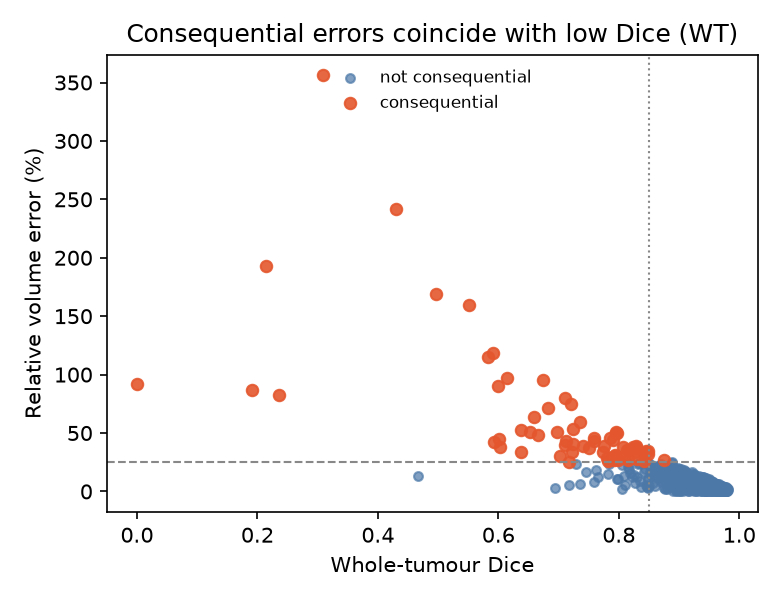
\includegraphics[width=\columnwidth]{fig1_dice_vs_volerr.png}
\caption{Consequential errors coincide with low Dice (whole tumour).}
\label{fig:1}
\end{figure}

\begin{figure}[t]
\centering
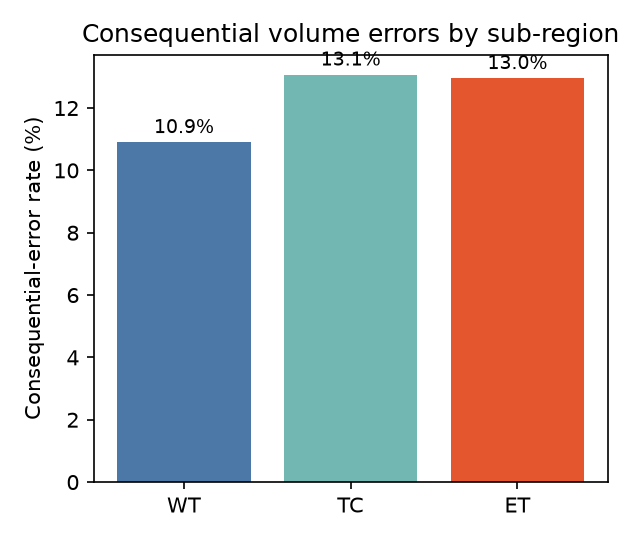
\includegraphics[width=\columnwidth]{fig2_rate_by_region.png}
\caption{Consequential-error rate by sub-region.}
\label{fig:2}
\end{figure}

\subsection{Consequence-flag vs.\ overlap-QC (A3/A4)}
\begin{table}[t]
\centering
\caption{WT primary endpoint on the frozen held-out \texttt{risk\_test}
($n{=}245$, $23$ positives). All methods are reference-free.}
\label{tab:flag}
\footnotesize
\begin{tabular}{@{}lccc@{}}
\toprule
Method & AUROC [95\% CI] & Retain @90\% & Residual \\
\midrule
best single uncertainty      & $0.838\ [0.744,\,0.916]$ & $56\%$ & $1.5\%$ \\
overlap-QC baseline          & $0.786\ [0.681,\,0.880]$ & $27\%$ & $3.0\%$ \\
predicted volume only        & $0.766\ [0.666,\,0.855]$ & $49\%$ & $1.7\%$ \\
\textbf{consequence flag} (ours) & $0.743\ [0.620,\,0.854]$ & $22\%$ & $3.8\%$ \\
\bottomrule
\end{tabular}
\end{table}

On the frozen held-out split (Table~\ref{tab:flag}) the consequence-targeted
flag ($0.743$) does \emph{not} beat the generic overlap-QC baseline ($0.786$) or
a \emph{single} uncertainty feature ($0.838$). \textbf{A4 verdict: pre-registered
null}---paired-bootstrap difference (consequence-flag $-$ overlap-QC) $=-0.043$,
$95\%$ CI $[-0.121,\,+0.019]$, $p{=}0.25$; consequence-targeting adds no
measurable value over generic reference-free QC. Practically, a simple
uncertainty check still enables useful triage: ${\sim}56\%$ of cases automated at
$90\%$ sensitivity with ${\sim}1.5\%$ residual consequential error on the
retained pile.

\section{Discussion}
\emph{Characterisation.} Consequential volume errors occur at ${\sim}9$--$13\%$
across sub-regions and are almost never silent---they coincide with low overlap,
and Dice is consistently and negatively coupled to relative volume error
($-0.63$ to $-0.81$).
\emph{Targeting hypothesis---refuted.} The consequence-targeted flag does not
beat generic overlap-QC or a single uncertainty feature (A4 difference $-0.043$,
$p{=}0.25$). For glioma, overlap quality already tracks clinical volume
consequence closely, so a generic reference-free QC suffices and a dedicated
consequence model is unnecessary---a useful, mildly counter-intuitive negative
result. Part of the coupling is mechanical (a large volume error forces low
overlap), which we state plainly rather than over-interpret.
\emph{Practical value.} Despite the null, a lightweight single-uncertainty check
safely automates ${\sim}56\%$ of cases at $90\%$ sensitivity with ${\sim}1.5\%$
residual consequential error---useful for deployment. Each of these is an
original, pre-registered finding, not a reused model.

\section{Limitations}
BraTS has one timepoint per patient, so the RANO-threshold analysis is a
single-timepoint simulation, not a real serial-scan decision. We use a single
segmentation architecture and one dataset family (BraTS), with no external-site
validation. Consequential cases are rare ($23$ WT positives on
\texttt{risk\_test}; $45$ on \texttt{risk\_dev}), so held-out AUROC confidence
intervals are wide (${\sim}\pm0.1$); development and held-out results agree,
which supports the null, but larger multi-centre cohorts would tighten the
estimates. Part of the overlap--volume coupling is mechanical (a large volume
error forces low Dice), so the ``no silent errors'' result is partly expected;
we report it as empirical confirmation, not a surprise.

\section{Conclusion}
We pre-registered and ran a reference-free study of \emph{clinically
consequential} glioma segmentation errors, with the headline evaluated once on a
frozen held-out split. Consequential volume errors in glioma are almost never
silent (they coincide with low overlap); targeting consequence therefore adds no
measurable value over generic reference-free QC (held-out A4 difference
$-0.043$, $p{=}0.25$)---a pre-registered null that refutes the
overlap-vs-volume-divergence assumption for this task; and simple reference-free
triage nonetheless safely automates ${\sim}56\%$ of volume measurements at $90\%$
sensitivity with ${\sim}1.5\%$ residual consequential error. The practical
takeaway: a lightweight overlap/uncertainty check is sufficient to triage
consequential glioma volume errors; a dedicated consequence model is not needed.

\begin{thebibliography}{5}
\bibitem{qcresunet}
P.~Qiu, S.~Chakrabarty, P.~Nguyen, S.~S.~Ghosh, and A.~Sotiras,
``QCResUNet: Joint subject-level and voxel-level segmentation quality
prediction,'' \emph{Medical Image Analysis}, 2025. arXiv:2412.07156.
\bibitem{confidence}
X.~C.~Wong, D.~Sarikaya, K.~Zucker, M.~De~Kamps, and N.~Ravikumar,
``Confidence is not reliability: Rethinking MC dropout in brain tumour
segmentation,'' arXiv:2606.19300, 2026.
\bibitem{metrics}
L.~Maier-Hein, A.~Reinke, \emph{et al.},
``Metrics Reloaded: Recommendations for image analysis validation,''
\emph{Nature Methods}, vol.~21, 2024.
\bibitem{rano2}
B.~M.~Ellingson \emph{et al.},
``A neuroradiologist's guide to operationalizing the RANO criteria version~2.0
for gliomas in adults,'' \emph{AJNR Am.\ J.\ Neuroradiol.}, vol.~45, no.~12,
pp.~1846--1856, 2024.
\bibitem{fneur}
``Response Assessment in Neuro-Oncology (RANO) review,''
\emph{Frontiers in Neurology}, 2026.
\end{thebibliography}

\end{document}
